%\documentclass[a4paper,conference]{IEEEtran}
%\documentclass[a4paper,10pt,conference]{ieeeconf}
%\documentclass[usletter, 10pt, conference]{ieeeconf}      % Use this line for a4 paper
%\IEEEoverridecommandlockouts                              % This command is only needed if 
%\overrideIEEEmargins                                      % Needed to meet printer requirements.

\documentclass{llncs}

\usepackage{graphicx}
\usepackage{booktabs}
\usepackage{amsmath}
\usepackage[ruled,lined]{algorithm2e}
\usepackage{multirow}
\usepackage[bookmarks=false]{hyperref}
\pdfminorversion=4

\newcommand{\red}[1]{\textcolor{red}{#1}}

\hypersetup{colorlinks=true,linkcolor=black,citecolor=black}

\SetKwInput{KwData}{Global params.}

\title{
    Analysis of protein tunnel traversability for flexible ligands using motion planning
}

\author{Vojt\v ech Von\' asek\inst{1} \and Barbora Kozl\'\i kov\'a\inst{2} \and Adam Jur\v{c}\'\i k\inst{2} \and Martin Saska\inst{1}}
\institute{
Faculty of Electrical Engineering,  
Czech Technical University in Prague, 
Technick\'a 2, 166 27, Prague 6, Czech Republic
\email{vonasek@labe.felk.cvut.cz}
\and
Faculty of Informatics,  
Masaryk University, 
Botanick\'a 68a, 602 00 Brno,
}


\def\qrand{q_{rand}}
\def\qstart{q_{start}}
\def\qinit{\qstart}
\def\qnear{q_{near}}
\def\qnew{q_{new}}
\def\C{\mathcal{C}}
\def\T{\mathcal{T}}
\def\CF{\mathcal{C}_{free}}
\def\Imax{I_{max}} %max number of iterations of RRT-based planners

\def\dist{\mathrm{dist}}
\def\dists{\mathrm{dist}_{\mathrm{s}}}

\SetKw{return}{return}

\def\VV{V_{vor}}
\def\VVA{V_{vor}^{act}}
\def\da{d_{high}}
\def\db{d_{low}}


\def\TA{$A_1$}
\def\TB{$A_2$}
\def\TC{$A_3$}

\def\probe{r_{\mathrm{probe}}}
\def\Sprobe{S_{\mathrm{probe}}}

\def\gprobe{r_{\mathrm{out}}}
\def\Sgprobe{S_{\mathrm{out}}}


\def\CG{\mathcal{C}_{goal}}
\def\SB{\mathbf{S}_{blocking}}
\def\SS{\mathbf{S}}

\def\RRTTD{RRT$_{\mathrm{td}}$}
\def\RRTN{RRT$_{\mathrm{n}}$}
\def\ths{d_\mathrm{surf}}

%spacing for algorithm environment. 1.0 mean normal spacing
\def\gb{p_{c}}

\begin{document}

\maketitle
%\frontmatter          % for the preliminaries


\begin{abstract}
%Proteins are involved in many biochemical processes.
Behavior and properties of proteins as well as other bio-macromolecules are influenced by internal void space such as tunnels or cavities.
%Behavior of proteins is influenced by internal void space such as tunnels or cavities.
Tunnels are paths leading from an active site inside the protein to its surface and they act as transporting pathways
to the active site.
To achieve a desired propery of the proteins, the active sites has to be reached by small molecules (ligands).
The widely used software tools for tunnel detection are based on Voronoi diagrams, which is suitable
for detecting tunnel of spherical probes.
It is however not easy to estimate if a given non-spherical ligand can pass a spherical tunnel.
Moreover, ligands are not rigid structures, but their conformation changes due to interactions with the protein's atoms.
In this paper, we propose to employ sampling-based motion planning techniques to analyze traversability of ligands in the spherical
tunnels.
To speed up the computation, the flexibility of ligands is modeled using a predefined set of conformations suitable (typical) for 
the given ligand.
We introduce a novel modification of RRT method, whose search in the corresponding configuration space is guided by
the tunnel pathway.
\end{abstract}

\section{Introduction}

Protein structures are essential components of all living organisms.
Proper understanding of their structure and function is important in many fields, including drug design, agriculture, cosmetics, etc.
Although this knowledge is still very hard to reveal, several protein structures have been already investigated in sufficient detail. % which led to their better understanding. 
Such investigation can incorporate computational methods which help to analyze the geometry of protein structure,  its shape, surface area, and inner void space. 
%These parameters then suggest and influence protein behavior, namely its reactivity with other molecules.
%consists of the analysis of protein structure, its shape, surface area, and inner void space. 
%These parameters influence namely the protein reactivity. % which is one of the most often studied behavior of the protein.


%Proteins interact with other molecules (small ligands, ribonucleic acid chains, other proteins, etc.) which can lead to changes in properties of the protein or the interacting molecule.
%Thanks to protein interaction with other molecules (small ligands, ribonucleic acid chains, other proteins, etc.), 
% we are able to change the properties of the protein or the interacting molecule. 
 For example, one task in protein engineering is to change selected properties of a protein, e.g. its stability under different outer conditions~\cite{Koudelakova2013} or activity of the protein towards the other molecules~\cite{Pavlova2009}.
%This is reached by studying so called tunnels in proteins which can serve as the transportation paths for the ligand from the outside environment to the active site or vice versa.
%For example, typical task in protein engineering is to change selected properties of a protein, e.g. its stability under different outer conditions [11] or activity of the protein towards other molecules [16]. 
This can be achieved by detecting and studying so called tunnels in proteins which can serve as the transportation paths for the 
ligand from the outside environment to the active site or vice versa. 
The active site is a specific site, usually deeply buried inside the protein, 
    where the chemical reaction between the protein and ligand can undergo. 
The importance of tunnels can be demonstrated on the study where mutations of amino acids located directly around the tunnel substantially improved the structural and kinetic stability of the studied protein, while
surface mutations almost did not contribute to the stabilization~\cite{Koudelakova2013}.

For example, one task in protein engineering is to change selected properties of a protein, e.g. its stability under different outer conditions~\cite{Koudelakova2013} or activity of the protein towards the other molecules~\cite{Pavlova2009}.
This is reached by studying so called tunnels in proteins which can serve as the transportation paths for the ligand from the outside environment to the active site or vice versa.
The active site is a specific site, usually deeply buried inside the protein, where the chemical reaction between the protein and ligand can undergo.
Since the importance of the presence of tunnels in proteins was revealed, the researchers started to study them intensively.
%Koudel\'{a}kov\'{a} et al.~\cite{Koudelakova2013} show that mutations of amino acids located directly around the tunnel improved the structural and kinetic stability of the studied protein substantially, while the surface mutations almost did not contribute to protein stabilization.
%The importance of tunnel can be demonstrated on an example, 
% where mutations of amino acids located directly around the tunnel improved the structural 
%and kinetic stability of the studied protein substantially, while surface mutations almost did not contribute to
%the protein stabilization~\cite{Koudelakova2013}.

The task of tunnel detection is to find a collision-free path leading from an active site inside the protein to its surface.
An example is depicted in Fig.~\ref{fig::motiv}.
As not all paths are biochemically relevant, only paths with a given minimal bottleneck have to be reported (the bottleneck is
the radius of the smallest sphere that can traverse the whole tunnel) 

Available tools for tunnel detection compute the tunnels assuming spherical ligands (probes). 
Bio-chemicists then decide if such a tunnel can be used to transport a given ligand mainly based on the tunnel
lengths and its bottlenect.
Such decision is however not precise and require previous expertise with the domain.

To provide more information about the traversability of the tunnels, it is necessary to consider a non-spherical model of 
the ligand.
Such task can be then solved using motion planning techniques.
It is necessary to consider translation, rotation and possibly also other degrees of freedom of the ligands, that are determined
by the torsional angles, the related configuration space, that need to be searched, is high-dimensional. 
Sampling-based motion planning techniques can be used to find a trajectory of the ligand.

Generally, the task of tunnel detection is to find a collision-free path leading from the active site to the protein's surface. 
The path is usually searched for a spherical probe of a given radius, which serves as a proxy geometry for a ligand. 
Early solutions focused on static molecules. 
However, from a static snapshot it is hard to assess the biochemical relevance of the tunnel as it does not
provide information about its temporal stability. 

Recently, researchers started to focus on molecular dynamics simulations and study the behavior of individual tunnels over time~\cite{yaffe2008,caver3,sehnal2013mole}.
%The path is searched for a spherical probe of a given radius.
%Early algorithms focused on static molecules, % and the tools were able to detect dozens of putative tunnels.
%but it was hard to assess their biochemical relevance because from a static molecule it is impossible to derive the temporal stability
%of the tunnels.
%Recently, researchers started to focus on molecular dynamics simulations and studying the behavior of individual 
%tunnels over time~\cite{yaffe2008,caver3,sehnal2013mole}.
Molecular dynamics is represented as a sequence of frames (molecule snapshots), and the tunnels need to be detected through these frames.
%With the increasing size of simulations the correctness of predicting the most biochemically relevant tunnel increases as well.
Existing solutions based exclusively on Voronoi diagrams and clustering methods are time and memory consuming
which also gives the limitation for the maximum number of frames which they are able to analyze.
In such cases, the biochemists have to select a subset of the whole simulation and perform the analysis only for this selection.
Such analysis however provides only a rough idea of the tunnel behavior, as important parts of the simulation can be easily omitted.
%This opens new possibilities for alternative solutions enabling to explore the tunnels in each frame of the molecular dynamics.
%In such cases the biochemists have to skip each n-th snapshot or select a subset of the whole simulation and perform the analysis only for this selection.
%Such analysis however provides only a rough idea of the tunnel behavior, as important parts of the simulation can be easily omitted. 
%Recently, we have proposed a novel method for tunnel detection using sampling-based motion planning [23]. In this method, RRT is used to ?nd tunnels in each frame and to consider the molecular dynamics, the tree is continuously pruned in each frame. In comparison to existing approaches [17], [18], this approach [23] handles the dynamics without need to cluster and match Voronoi diagrams from consecutive frames. 


Curently available tools for protein analysis support only the tunnel detection both on single protein snapshots and sequences
of molecular dynamics.
The properties of tunnels like bottleneck radius, their length and the surrounding residues can be used
to estimate suitability of the tunnel for a ligand.
However, such estimation still involve lot of experience.

\red{TODO}
something about screeing: what is it, what's is the input and output, in which applications (research/industry) it is useful.



\begin{figure}[t]
\centering
{\footnotesize
\renewcommand{\arraystretch}{0.1}
\renewcommand{\tabcolsep}{0pt}
\begin{tabular}{ccc}
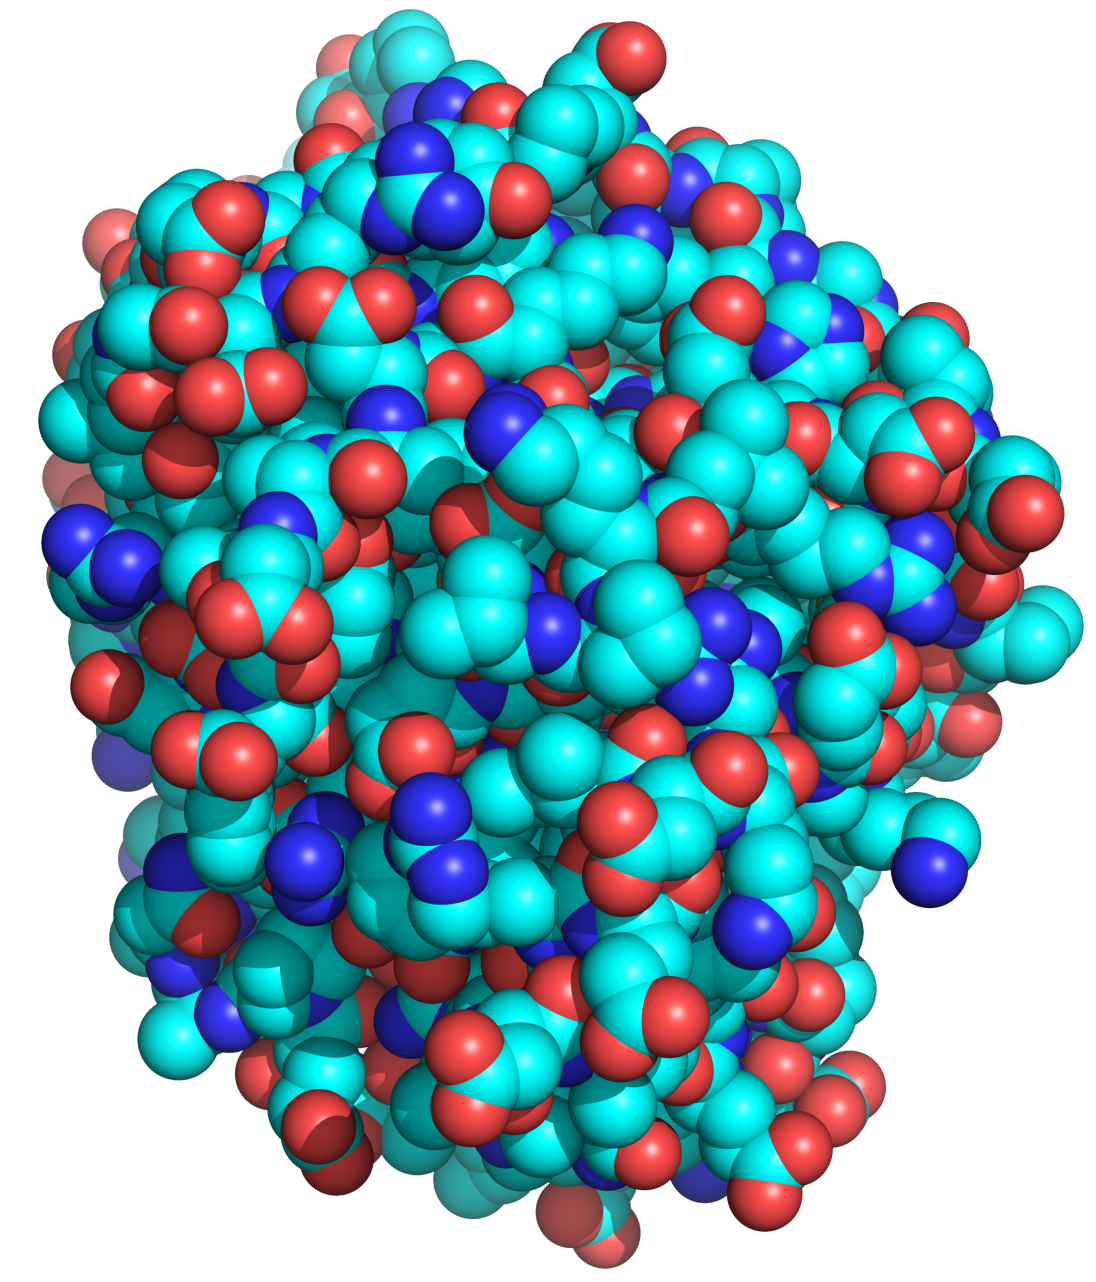
\includegraphics[width=0.15\textwidth]{fig/motiv1} &
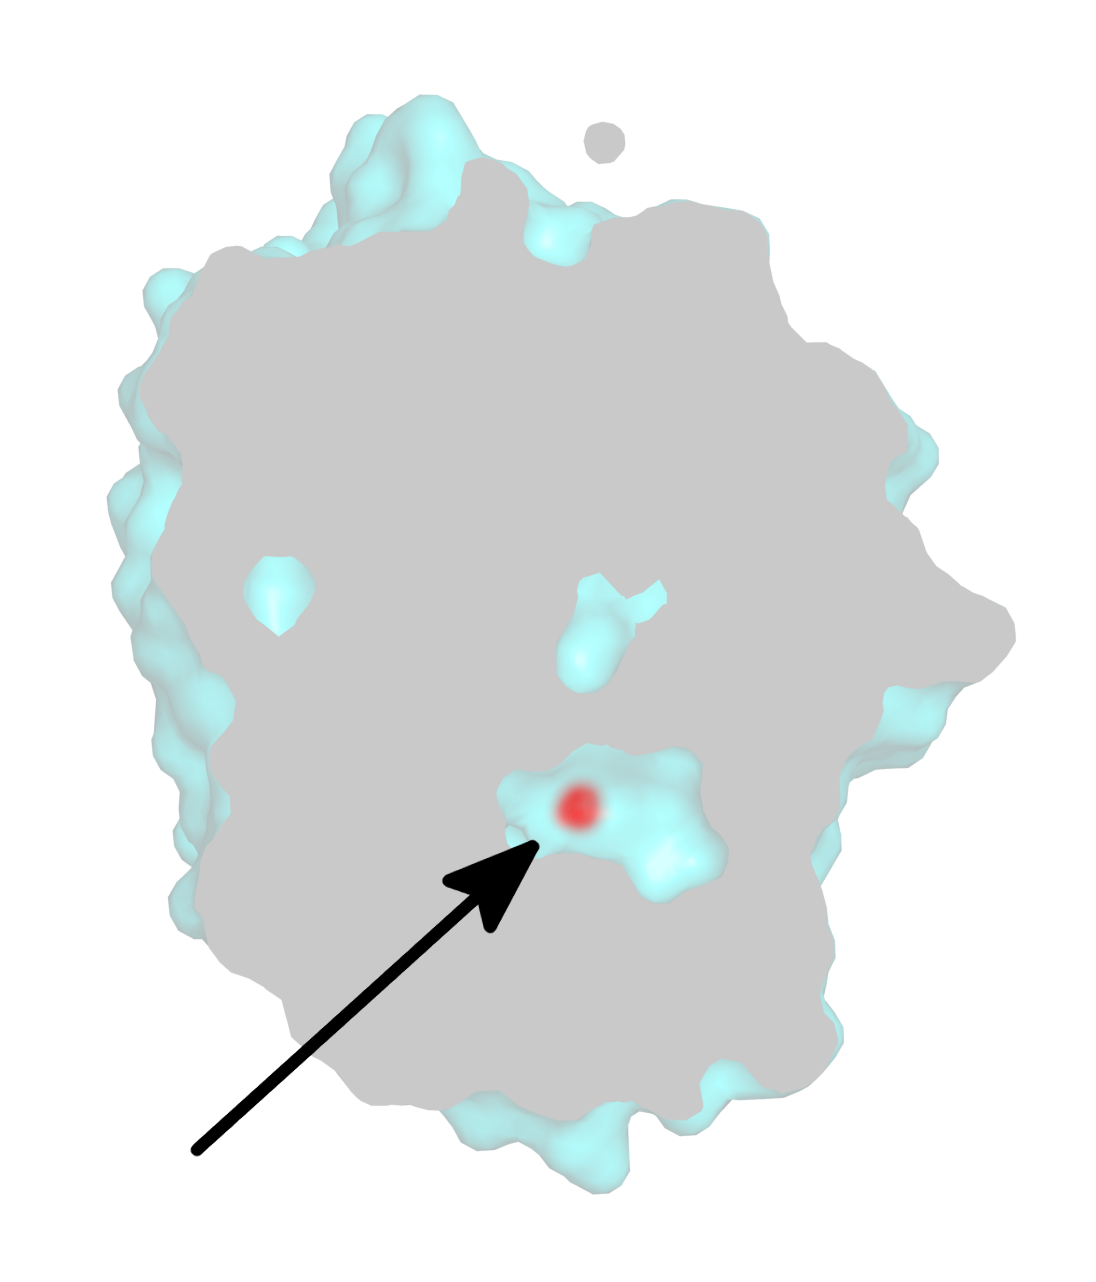
\includegraphics[width=0.17\textwidth]{fig/motiv2lab} \\
%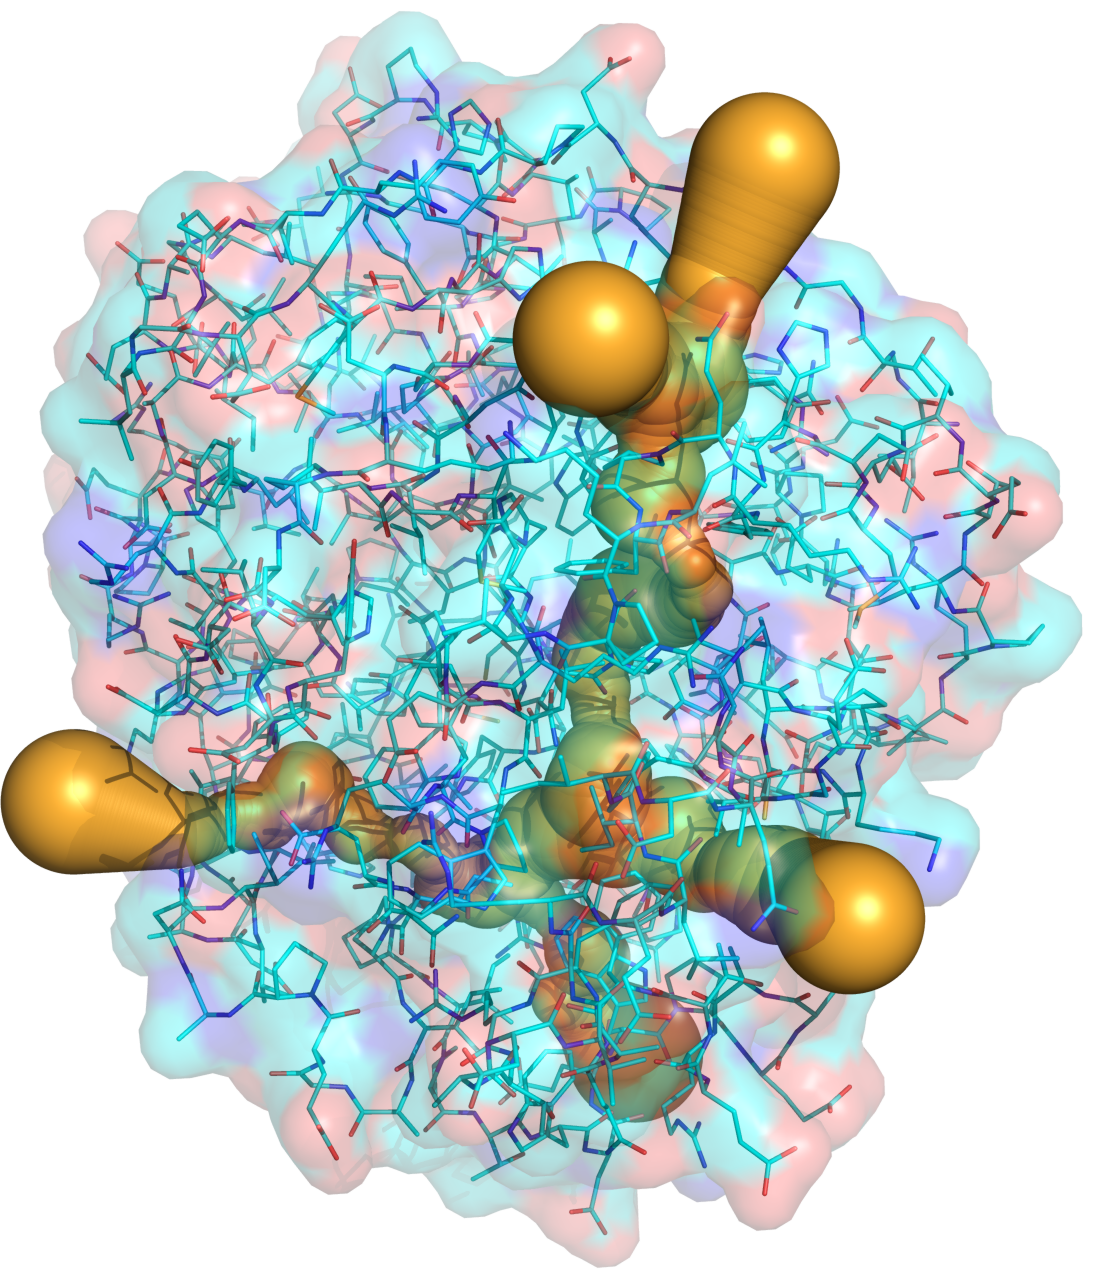
\includegraphics[width=0.16\textwidth]{fig/motiv3} \\
Protein 1CQW & Active site & Detected tunnels \\
             &            & (orange)
\end{tabular}
}
\caption{\label{fig::motiv}
    Example of tunnel detection in haloalkane dehalogenase.
}
\end{figure}

\red{TODO}
what is traversability analysis.

The goal is the traversability analysis is to estimate traversability of a tunnel with a given ligand from geometrical point of view.




\section{Related work}

\red{TODO include}
Recently, we have proposed a novel method for tunnel detection using sampling-based motion planning, namely using Rapidly Exploring Random Tree (RRT) method~\cite{vonasek2016application}.
In comparison to existing approaches~\cite{Petrek20071357,citeulike:6257975}, this RRT-based approach~\cite{vonasek2016application} 
handles the dynamics without need to cluster and match Voronoi diagrams from consecutive frames.


The analysis of protein structure aiming to reveal the tunnels has been supported by different computational software tools which take the geometry of the protein as an input and explore the inner void space (e.g., CAVER 1.0~\cite{citeulike:6257975} or MOLE~\cite{Petrek20071357}). 
Early methods for tunnel detection utilized a discretized 3D grid, where each cell is considered as occupied or free depending
on the presence of atoms of the protein.
Tunnels can be then searched using standard graph-search methods like Dijkstra's algorithm.
Besides, the grid can be used to identify other relevant properties like 
pockets, cavities, or channels~\cite{sehnal2013mole,citeulike:6257975}.
%One of the first grid-based approaches to the detection of tunnels in protein is the CAVER 1.0 algorithm by Pet\v{r}ek et al.~\cite{citeulike:6257975}.
The obvious disadvantage of the grid-based methods is the high memory demand and their dependency on the grid resolution.
Due to the high memory consumption, these methods are not suitable for tunnel detection in dynamic proteins and therefore they
are used primarily for analysis of static molecules or individual snapshots of dynamics.

%hese approaches are not suitable for tunnel detection in dynamic proteins, a
%, which limits the usage of these methods for spherical ligands.
%To increase precision by 10, the number of cells increases by $10^3$.
%Another disadvantage is that the 3D grid does not consider orientation of the ligand and therefore, the computations 
%are useful only for spherical ligands.

Currently the most widely used approach to tunnel detection is based on Voronoi diagrams (VD) or Weighted Voronoi Diagrams (WVD).
The ordinary VD is computed on points representing centers of all atoms, without considering radii of the atoms.
This may lead to detection of tunnels with incorrect bottlenecks. % i.e., incorrect radius of a smallest probe that can traverse the tunnels.
To consider atoms with different radii, weights of individual points are determined by the van der Walls radii of the atoms in WVD.
An alternative solution is to compute a non-weighted VD on an extended point set, where 
each atom is approximated by several spheres with small radius~\cite{yaffe2008,caver3}.
%In this case, each atom is approximated by several spheres with small radius~\cite{yaffe2008,caver3}.
%The VD-based methods remove one of the main limitations of the grid-based approach which is the dependency on the grid resolution.
VD-based methods are memory less demanding, and also faster than grid-based methods.
%They can be easily used for static tunnel detection, as they are based on Voronoi diagrams of static frames.
%The grid-based and VD-based methods are usually employed on static proteins.
%Finding tunnels through time-changing proteins increases the dimension of the space to be searched, which prevents the grid-based methods
%to be used for this task.
The extension of VD-based methods to dynamic molecules requires to construct VD in the frames being analyzed and 
finding correspondences between them.
The existing approaches often use hierarchical clustering to match Voronoi vertices and edges from different frames, which is computationally demanding~\cite{lindow2012dynamic,caverDetails}.
%The main limitation of this approach is that this solution builds a complex and large hierarchical tree which has to be stored in memory and subsequently traversed which is computationally demanding. %~\cite{lindow2012dynamic}.


The tunnel detection in dynamic proteins can also be formulated as path planning in 4D (i.e., 3D $\times$ time) 
configuration space assuming a spherical probe.
%Tunnel detection in dynamic proteins leads to path planning 
%in a high-dimensional configuration space (4D for the probe and 7D for the ligand).
This space can be searched using sampling-based motion planning methods.
%Instead of a systematic search, which would be time and memory consuming, randomized sampling can be used
%to obtain necessary information about the configuration space. %~\cite{Lav06}. 
%Path planning approaches studied in robotics can be used to solve tunnel detection~\cite{guieysse2008structure} as well.
%Sampling-based path planning methods like Probabilistic Roadmaps (PRM)~\cite{kavrakiPRM} and Rapidly Exploring Random Trees (RRT)~\cite{lavalleRRT} are able to find feasible paths for complex objects with arbitrary geometries.
The idea of sampling-based motion planning is to randomly sample the configuration space $\C$ of the robot. % (i.e., the spherical probe in this case).
%The configuration space is a space of all possible configurations of the robot.
The random samples are classified as free or non-free using collision detection and  the free ones are stored into a roadmap.
A path in the roadmap then represents a motion in the workspace.
%The usage of collision detection for classification of samples allows the application of sampling-based methods for path planning for robots (objects) of arbitrary shapes.
%As the sampling-based methods work in the configuration space, they can cope with objects (robots) of many degrees of freedom
% and arbitrary shapes.
%Sampling-based planners have been used in various applications in robotics~\cite{elbanhawi2014sampling} and also  %,latombe1999motion} and also
% to study proteins, e.g. in  
%loop motions~\cite{cortes2004geometric},
%protein folding~\cite{amato2002using,raveh2009rapid,novinskaya2015improving,songPFintro},
%protein folding~\cite{raveh2009rapid,novinskaya2015improving},
%or protein folding combined with ligand diffusion~\cite{cortes2010simulating}.
Rapidly Exploring Random Tree (RRT)~\cite{lavalleRRT} is a single-query motion planning method.
RRT incrementally builds a configuration tree $\T$ rooted at the initial configuration.
In each iteration of RRT, a random configuration $\qrand \in \C$ is generated and its nearest node in the tree $\qnear \in \T$ is found.
A new configuration $\qnew$ is constructed on the line connecting $\qnear$ and $\qrand$ in the distance $\varepsilon$.
If $\qnew$ is collision-free, it is added to the tree.
The algorithm terminates if the tree approaches the goal configuration close enough.

Beyond robotics, sampling-based motion planners have been successfully applied in computational biology in studies
related to 
protein folding~\cite{al2012motion,gipson2012computational,cortes2010simulating,amato2002using,raveh2009rapid,novinskaya2015improving,songPFintro}, or analysis of loop motions~\cite{cortes2004geometric}.
%rrt for molecular: \cite{al2012motion}
%survey \cite{gipson2012computational}
Solutions for tunnel detection using sampling-based methods however have not been discussed yet.
The most relevant paper is~\cite{guieysse2008structure}, where RRT is used to compute pathways for flexible ligands towards 
the active site.
This method however does not compute explicitly all tunnels, rather a single pathway.

In our recent paper~\cite{vonasek2016application}, we have proposed to detect tunnels using RRT.
In this approach, RRT samples the configuration space of a small spherical probe moving in a single frame of protein dynamics.
After the tunnels are found in one frame, the built  configuration tree is transferred to the next frame of protein dynamics and pruned to remove
nodes colliding with the new positions of atoms.
This results in a sequence of connected trees, that can be searched for path representing the tunnels in the protein dynamics.

%This allows us to build a sequence of trees, where each tree corresponds to each frame of protein dynamics.
%The nodes of the trees are connected to their parents in the same frame, or to their parents in the previous frame.
%This allows us to find paths in this sequence of tree between two given frames, that correspond to the dynamic tunnels.

In comparison to~\cite{guieysse2008structure}, the approach~\cite{vonasek2016application} assumes spherical probes, which is motivated
by practical reasons.
%The tunnels can be computed for a spherical probe or even for non-spherical ligands --- small molecules.
%Computing tunnels considering only spherical probes is more practical.
%Despite the ability of sampling-based planners to find path for robots (objects) of arbitrary shapes, which is achieved by the collision detection, the above described approach~\cite{vonasek2016application} detect tunnels only for spherical ligands.
%The reasons are practical.
Flexible ligands have many degrees of freedom, which increases dimension of the configuration space to be searched and makes
the collision-detection more complex.
Moreover, it is required to define suitable metric and possibly also an efficient data structure for nearest-neighbor search.
%Dimension of the configuration space of flexible ligands is higher and it is determined by the Degrees Of Freedom of the ligand.
%It is required to define proper metric to efficiently search this space using RRT.
%Planning patways for flexible ligands leads to a search in a high-di
%Taking into account flexible ligands increases the dimension of the configuration space.
Despite the flexibility of ligands, their movements in proteins are strongly limited, as they are typically larger than spherical
probes.
Traversability of the ligand through a protein may depend on its initial orientation, 
 which can further limit the growth of the configuration tree.
Contrary, configuration space of  spherical probes is only 3D with the possibility to employ Euclidean metric and KD-trees for the
nearest neighbor search.
It is more practical to first detect tunnels for a spherical probe and then analyze traversability of the actual shape of ligand.
In this case, the traversability analysis is limited only to a tunnel and its vicinity, which decreases volume of the configuration space and
decreases the number of atoms involved in collision detection.
%which is faster than searching path for the ligand in the full protein.

%The ability of RRT to quickly explore the configuration space is caused by the combination
%of uniform sampling and the nearest-neighbor rule used to select nodes for the expansion.
The growth of the configuration tree into some regions of the configuration space can however be slowed down due to the narrow passages.
A narrow passage is a small region of the configuration space containing part of the solution.
As the samples are generated from uniform distribution in RRT, probability of placing the samples into the narrow passages is low and therefore,
   the probability of expanding the tree through a narrow passage is small~\cite{hannaWIS}.
%Due to its low volume, the probability of expanding the nodes towards the passage is small~\cite{hannaWIS}.
%    many iterations are needed before a tree can be built through the passage~\cite{hannaWIS}.

A possible solution is to estimate the location of narrow passages from the knowledge of the workspace and generate more samples
in the difficult areas.
For Probabilistic Roadmaps~\cite{kavrakiPRM}, this can be achieved simply by generating more samples in the difficult areas, e.g. along
medial axis~\cite{wilmarthMAPRM,foskey01hybrid,guibas1999probabilistic,hoff2000interactive,yang2004adapting}.
%This requires to precompute the medial axis, which can be time consuming.
%Another approach is to shift the random samples towards the medial axis~\cite{amatoOBPRM} or into a direction of estimated
%medial axis~\cite{hollemanMAPRM}.
Generating random samples in difficult regions however does not ensure construction of a better tree in the case of RRT-based methods. 
In RRT, the configuration tree is expanded in the direction of random samples, but the obstacles may prevent to reach them closely~\cite{vonasekphd}.
Increased probability of sampling in a given region, e.g., in a narrow passage, 
brings advantage only if the tree is close to the region and if it can reach it.
To utilize a knowledge about the environment in the sampling process, represented e.g. using a mexial axis or a 2D or 3D path,
it is necessary to maintain the sampling regions according the progress of the tree.
For example, random samples can be generated along a given workspace path~\cite{vonasek2009rrt}.
After the tree reaches a path point, the sampling around the point is disabled and moved to the next point of 
the path.
Similarly in
\cite{jorry14marrt,neddy2016dynnamic}
ob-rrt
rrt-retraction


In this paper, we propose how to combine RRT-based search with Voronoi-based methods in the task of tunnel detection. 
To guide the configuration tree using Voronoi diagram, a subset of Voronoi vertices is determined and
the samples are generated around vertices in this subset.
The subset is maintained according the distance from the tree, so the random samples
are generated only if they are in a suitable distance from the tree.
This allows us to sample simultaneously along all promissing parts of VD that are accessible from the tree, which is 
suitable for detection of multiple tunnels.


%In this paper, we propose how to combine the VD-based methods and sampling-based approaches for tunnel detection.
%Instead of uninformed sampling of the configuration space, which has been proposed in~\cite{vonasek2016application}, we propose
%to generate the random samples using Voronoi diagrams.


%~\cite{amatoOBPRM,hollemanMAPRM} shift random samples towards medial axis of the environment, which helps to sample
%narrow passages more densely. 
%For example, the random samples generated in the configuration space can be shifted
%towards the medial axis of the environment~\cite{amatoOBPRM,hollemanMAPRM} or even generated around the medial 
%axis~\cite{wilmarthMAPRM,foskey01hybrid,guibas1999probabilistic,hoff2000interactive,yang2004adapting}.
%The paper~\cite{amatoOBPRM} suggests to sample uniformly in the configuration space and shift the samples towards the medial axis.
%Another approach is to generate the samples randomly in \CS\ and shift them closer to the medial axis~\cite{amatoOBPRM}.
%The medial axis can be computed exactly using GVD.
%While the medial axis can be easily computed for 2D or 3D workspaces using GVD, its computation become complicated in many dimensions.
%In such case, the samples can be generated uniformly from the whole \CS\ and moved in an estimated direction towards the medial axis~\cite{hollemanMAPRM}.



%sampling-based for 
%protein-ligand access and docking \cite{bayazit2001ligand,singhLig,apaydin2004stochastic,cortes2010simulating}
%protein and RNA folding~\cite{amatoPF1,ApaBru03}
%protein loop motions~\cite{cortes2004geometric},
%domain motions~\cite{kirillova2008an}, 
%and motions of pairs of alpha-helices in transmembrane proteins~\cite{enosh2007prediction}

%The tree is extended from a node, that is selected as a nearest node to a randomly generated configuration in the configuration space.
%The highest probability of expansion have nodes with large Voronoi cells. 
%Due to this Voronoi-bias, the tree grows towards unexplored regions of the configuration space.
%However, the Voronoi-bias brings disadvantages in narrow passages.
%nodes in the narrow passages.



%The behavior of RRT in the narrow passages was analyzed using Voronoi diagrams in~\cite{yershovaDDRRT}.
%The nodes in the tree can be divided into two groups: frontier nodes, whose Voronoi cells grow together with growth
%of the environment and boundary nodes, which are close to the obstacles. %~\cite{yershovaDDRRT}.
%The tree cannot be expanded from the boundary nodes.
%In a narrow passage, the nodes are both boundary and frontier.
%These nodes are frequently selected for the expansion, because they are the frontier nodes, however the tree cannot be expanded
%from them, because they are also the boundary nodes. 
%To suppress selection of the boundary nodes, authors of~\cite{yershovaDDRRT} suggest to define an action radius around each node.
%The node is selected for the expansion only if its radius is larger than the distance to the random sample.
%The radius of new nodes is set to $\infty$ and it is decreased to a predefined value $\rdd$ if the node cannot be expanded.
%A Dynamic-Domain strategy for RRT (RRT--DD) is proposed in~\cite{yershovaDDRRT}:
%each node holds an action radius defining how far can be a random sample $\qrand$ that activates the node for the expansion.
%The RRT--DD algorithm generates random samples $\qrand$  and finds its nearest neighbor in the tree
%$\qnear$ until $\rho(\qrand,\qnear) < \qnear.radius$. 
%Although the algorithm is efficient in the narrow passages, it is strongly influenced by the parameter $\rdd$.
%To decrease the sensitivity of the method to the parameter $\rdd$, it can be automatically adjusted, which
%was proposed in RRT--ADD (RRT with Adaptive Dynamic Domain)~\cite{jailletATDDRRT}.
%Another schema to automatically adjust parameters of the RRT-based planners was proposed in~\cite{schneider2015completely}.

%Retraction-RRT~\cite{zhangRetraction} generates random samples uniformly as in the original RRT, but it
%attempts to shift them into the narrow passages.
%A~random configuration $\qrand \in \CF$ is generated and a close non-free configuration $q \in \CO$ is found. 
%A~contact configuration $q_c$ on a segment $(\qrand,q)$ is found and its neighborhood is searched for
%$q_c'$ minimizing the distance between $q$ and $q_c'$. 
%The configuration $q_c'$ is then added to the tree.
%It was shown that this approach can deal with narrow passages efficiently,
%because the generated contact configurations penetrate into the narrow passages.
%However, to find the contact configurations, the collision detection algorithm is called frequently, which can decrease
%the performance of the algorithm.

%The goal-bias principle can be further extended by sampling the configuration space along a path computed in the workspace~\cite{vonasek2009rrt,amatoOBRRT}.
%%Geometric path in the workspace~\cite{vonasek2009rrt} or medial axis of the 3D space~\cite{amatoOBRRT} can be used to guide the tree.
%Sampling along geometric paths constructed in the workspace is suitable for low-dimensional configuration spaces, e.g. for
%path planning of mobile robots.
%However, the geometric paths computed in workspace are less effective for sampling in high-dimensional configuration spaces~\cite{hannaWIS}.
%



%of the narrow passages is related to narrow passaged of the workspace~\cite{hannaWIS}.
%
%is to manipulate the random samples, e.g. to change their rotation, rotation or both parts or to shift them closer to the medial
%axis of the workspace~\cite{amatoOBPRM}.

%In~\cite{amatoOBPRM} several strategies for validating non-free random samples have been proposed.
%Authors propose different manipulation procedures for random configurations generated during the learning phase.
%For example, the random configuration can be placed into the roadmap with changed rotation, translation or both, or it can be
%shifted away from an obstacle allong a line connecting the sample and medial axis of the obstacles.
%In a configuration is invalid, it is pushed randomly into various directions to gen free samples around boundaries of $\CO$.





% ===============================================================================


%25\% of VDW radii, T-RRT \cite{jaillet10costmap}

%\red{The tunnel detection task differs from classic motion planning it two main aspects: a) the goal configuration
%is not explicitly defined, and b) multiple pathways (tunnels) should be detected.}


%Molecular structures can be represented as articulated bodies and sampling-based methods can be used
%Path planning methods have been used to expore the conformational space of 
%proteins~\cite{novinskaya2015improving,songPFintro,mollProt,proteinRRT},
%Other applications of sampling-based approaches is in detection of 
%folding pathways~\cite{amato2002using}, analyzing protein loops~\cite{cortes2004geometric}, 
%or modeling large-scale transitions in a protein structure~\cite{raveh2009rapid}
%The geometric-based tunnel detection approaches provide fast computation of tunels in large protein structures and they
%have been integrated in several tools like Caver~\cite{bara2014caver}, Chexvis~\cite{masood2015chexvis} and other.
%Most of the proposed methods consider only spherical models of ligand~\cite{benkaidali2014computing}.

%dxTuber: Detecting protein cavities, tunnels and clefts based on protein and solvent dynamics:
%furtng protein cavities, tunnels and clefts based on protein and
%solvent dynamics insights into the protein in question. For example, empty
%space in a protein structure can provide valuable insight into protein properties such as internal hydration, structure stabilization,
%substrate translocation, storage compartments or substrate binding sites [1,2]. This information can be visualized by means of cav-
%ity analysis. Over the years numerous cavity detection tools have been developed including [3–17] that depict cavities either directly
%[3–6,8,10–17] or indirectly by identifying lining residues [9] or filling a cavity with water molecules [7]. The main strategies used
%in these geometry-based algorithms [1] can be grouped into four categories plus combinations of these.
%n the motion planning problem, that is widely studied in robotics, the task is to find a feasible trajectory for a robot between two

%given positions in an enironment.
%To utilize the motion planning approaches, the ligand is considere as the robot and the protein's atoms as the obstacles.
%Computing feasible (traversable) tunnels for non-spheric ligands requires to consider also rotations of the ligands, which 
%can be solved using sampling-based approaches like Probabilistic Roadmaps (PRM)~\cite{kavrakiPRM} or Rapidly Exploring
%Random Trees (RRT)~\cite{lavalleRRT}.
%Sampling-based methods randomly samples configuration space of the robot (ligand) and the samples are classified
%as free or non-free using collision detection.
%The free samples are stored in a graph structure.
%A path in the grap then corresponds to a motion in the workspace.



%In~\cite{guieysse2008structure}, RRT method is used to compute pathways for flexible ligands.


%\cite{lindow2012dynamic}
%Analysis of protein dynamics suggests that internal cavities and channels can be rather dynamic structures. 
%Voronoi-based algorithm to extract the geometry and the dynamics of cavities and channels from a molecular dynamics trajectory.
%The algorithm requires a pre-processing step in which the Voronoi diagram of the van der Waals spheres is used to calculate the cav-
%ity structure for each coordinate set of the trajectory. 
%In the next step, we interactively compute dynamic channels by analyzing the time evolution of components of the cavity structure. Tracing of the
%cavity dynamics is supported by timeline visualization tools that allow the user to select specific components of the cavity structures
%for detailed exploration. All visualization methods are interactive and enable the user to animate the time-dependent molecular struc-
%ture together with its cavity structure. To facilitate a comprehensive overview of the dynamics of a channel, we have also developed a
%visualization technique that renders a dynamic channel in a single image and color-codes time on its extension surface. 
%
%
%Sampling-based motion planning algorithms from the field of robotics have been very successful in exploring the
%conformational space of proteins
%\cite{novinskaya2015improving}
%Sampling-based algorithms explore the conformational space of a protein by randomly sampling it (usually using a special
%heuristic) and constructing a graph where each node represents a feasible low-energy protein conformation (or state), and each
%edge represents a possible low-energy local transition between two states. 
%The computed graph describes the topology of a protein’s energy landscape and the connectivity of its lowenergy areas. 
%This graph can be used to find possible large-scale transitions between two given protein conformations.
%

%Sampling-based methods have been very effective for the fast computation of representative motions of molecular systems \cite{al2012motion, gipson2012computational}


%A broad range of approaches exploit sampling-based techniques to address various biological problems, such
%as exploring energy landscapes \cite{devaur2014sampling} ,
%modeling protein folding pathways \cite{amato2002using}, analyzing protein loops \cite{cortes2004geometric}, 
%or modeling large-scale transitions in a protein structure \cite{raveh2009rapid}

%In computational biology, molecules and proteins are modeled as articulated bodies and sampling based planners are used to simulate
%protein folding and protein-ligand interactions  \cite{al2012motion} 
%asi spis necitovat \cite{gipson2012computational}



%Ms have been applied to model molecular motions by modeling the molecule as an articulated linkage and 
%replacing the typical collision detection validity check with some measure of physical viability (e.g., potential energy).
%Protein motions, ranging from molecular flexibility to large-scale conformational change, play an essential role in many biochemical processes. 
%!!to map transitinos between specific conmfotrmations!!!!
%ample conformation space more effectively, and we describe extensions of our framework to automate
%the process and to map transitions between specified conformations.
%\cite{thomas2006simulating}
%

%In subsequent work, our group used another PRM variant on this problem \cite{bayazit2001ligand}
%Our group was the first to adapt PRMs to model protein folding pathways 
%\cite{amato2003using, amato2002using, song2003apath}

%Using a standard modeling assumption for proteins that bond angles and bond lengths are fixed \cite{sternberg1996protein}, 
%the only dof in our model are the backbone’s phi and psi torsional angles which are modeled as revolute joints with values 0 .. 2pi

%
%The roadmap produced by our technique is an approximation of the protein’s energy landscape. 
%Roadmap quality is measured both by how realistic (as compared to experimental data) its pathways are and by how many samples are required
%to achieve the desired accuracy. 
%The latter is important because it determines what size molecules can be analyzed.
%Hence, sampling is the key to producing a good approximation of the land-scape. 
%Note that only a relatively small portion of the conformation space ‘near’ the target conformation(s) is of interest in modeling motions. 
%This implies that we should use biased sampling to cover the regions of interest efficiently.
%
%genrovani lepsich vzorku: using rigidity analysis~\cite{thomas2006simulating}
%or perturbing:
%iterative sampling process where we apply small Gaussian perturbations to existing conformations~\cite{amato2003using, amato2002using, song2003apath}
%
%rrt for tunnel (pathway) detection
%\cite{cortes2010simulating}
%\cite{corset2005path}
%\cite{guieysse2008structure}
%

%Many modifications have been proposed for RRT to speed up the growth of the tree~\cite{kuffnerRRTC}, 
%     to consider an optimality criteria such as path length~\cite{karaman2011sampling}, and to improve behavior in narrow passages~\cite{amatoOBRRT,vonasek2009rrt,zhangRetraction,schneider2015completely}. 
%For example, RRT--Retraction~\cite{zhangRetraction} analyzes the line segment from $\qnear$ to $\qrand$.
%If the line segment is collision-free, the tree is expanded normally using the straight-line planner.
%Otherwise, the contact configuration on the line segment is constructed and its neighborhood is searched
%for other contact configurations in order to minimize the distance to $\qrand$.
%This retraction step allows RRT--Retraction to place the nodes of the tree into narrow passages.



%The behavior of RRT in the narrow passages was analyzed using Voronoi diagrams in~\cite{yershovaDDRRT}.
%The nodes in the tree can be divided into two groups: frontier nodes, whose Voronoi cells grow together with growth
%of the environment and boundary nodes, which are close to the obstacles. %~\cite{yershovaDDRRT}.
%The tree cannot be expanded from the boundary nodes.
%In a narrow passage, the nodes are both boundary and frontier.
%These nodes are frequently selected for the expansion, because they are the frontier nodes, however the tree cannot be expanded
%from them, because they are also the boundary nodes. 
%To suppress selection of the boundary nodes, authors of~\cite{yershovaDDRRT} suggest to define an action radius around each node.
%The node is selected for the expansion only if its radius is larger than the distance to the random sample.
%The radius of new nodes is set to $\infty$ and it is decreased to a predefined value $\rdd$ if the node cannot be expanded.
%A Dynamic-Domain strategy for RRT (RRT--DD) is proposed in~\cite{yershovaDDRRT}:
%each node holds an action radius defining how far can be a random sample $\qrand$ that activates the node for the expansion.
%The RRT--DD algorithm generates random samples $\qrand$  and finds its nearest neighbor in the tree
%$\qnear$ until $\rho(\qrand,\qnear) < \qnear.radius$. 
%Although the algorithm is efficient in the narrow passages, it is strongly influenced by the parameter $\rdd$.
%To decrease the sensitivity of the method to the parameter $\rdd$, it can be automatically adjusted, which
%was proposed in RRT--ADD (RRT with Adaptive Dynamic Domain)~\cite{jailletATDDRRT}.
%Another schema to automatically adjust parameters of the RRT-based planners was proposed in~\cite{schneider2015completely}.

%Retraction-RRT~\cite{zhangRetraction} generates random samples uniformly as in the original RRT, but it
%attempts to shift them into the narrow passages.
%A~random configuration $\qrand \in \CF$ is generated and a close non-free configuration $q \in \CO$ is found. 
%A~contact configuration $q_c$ on a segment $(\qrand,q)$ is found and its neighborhood is searched for
%$q_c'$ minimizing the distance between $q$ and $q_c'$. 
%The configuration $q_c'$ is then added to the tree.
%It was shown that this approach can deal with narrow passages efficiently,
%because the generated contact configurations penetrate into the narrow passages.
%However, to find the contact configurations, the collision detection algorithm is called frequently, which can decrease
%the performance of the algorithm.


%Another approach to biased sampling was presented in~\cite{bruceERRT}, where the trajectories found in previous
%iterations are used to sample the configuration space. 
%This modification is suitable for dynamic environments.

%The growth of the tree can be attracted into a region $\R \in \C$ by increasing probability of sampling in that region.
%This is used in the goal-bias principle~\cite{lavalleRRTPP}, where $\qgoal$ is used instead of $\qrand$ with the probability $\gb$.
%The goal-bias suppresses the exploration of $\C$ and the tree is expanded more preferably towards the goal.
%An extension of the goal-bias was presented in~\cite{kardossRRTKK}, where a predefined key-configuration is 
%used to focus sampling to difficult areas of the configuration space.
%%Authors suggest to place the key-configuration in a way that connects easy and difficult areas of the configuration space.
%%For example, the key-configuration can be placed at the enter to a narrow passage.
%%Although the goal-bias speeds up the growth towards the goal, it may cause a congestion problem of the tree growth due to existence of an obstacle in the pathway.
%
%
%The goal-bias principle can be further extended by sampling the configuration space along a path computed in the workspace~\cite{vonasek2009rrt,amatoOBRRT}.
%%Geometric path in the workspace~\cite{vonasek2009rrt} or medial axis of the 3D space~\cite{amatoOBRRT} can be used to guide the tree.
%Sampling along geometric paths constructed in the workspace is suitable for low-dimensional configuration spaces, e.g. for
%path planning of mobile robots.
%However, the geometric paths computed in workspace are less effective for sampling in high-dimensional configuration spaces~\cite{hannaWIS}.
%


\section{Preliminaries}

Proteins are represented by the hard sphere model, where the radius of each sphere (atom) is given by its van der Waals radius.
Let $\SS \subset \mathbf{R}^3$ denote the union of all spheres, i.e., the geometry of the protein.
%We further assume that a subset of atoms located at the surface, are known. These atoms, reffered to as {\sl surface atoms} in this paper,
%   can be detected as atoms located at $\alpha$-shape of the molecule.
The tunnels need to be found for a spherical probe $\Sprobe$ of radius $\probe$.

A tunnel is described by a sequence of collision-free spheres $T=( (t_i, r_i) )$, where $n$ denotes the number of spheres and
$t_i=(x_i,y_i,z_i)$ is their 3D position and $r_i$ denotes the maximum collision-free radius for a spherical probe centered
at $t_i$. 
The tunnels can be found by tunnel-detection tools like CAVER 3.0~\cite{caver3}.

Ligands are small molecules interacting with the protein. 
Due to the interaction, the relative positions of the ligand's atoms can change.
the ligands  can be modeled as a multi-link kinematic chain where the torional angles phi/psi can change in a given range~\cite{songPFpath}.
After the torsional angles are set, 3D position of each atom of the ligand is computed.
By changing the angles, various conformations can be generated.
However, not all conformations are feasible, which has to be checked using potential energy, which is time consuming.

To decrease the computational burgen, a set of feasible conformations $C$ is prepared.
The conformations can be prepared using Molecular Dynamics software such as Rosetta.
For each conformation $c\in C$ an energy potential is also calculated.
The transition matrix $M$ defines the possible changes of conformations, i.e., $M(i,j)=1$ if the conformation $c_i \in C$
can be switched to the confomration $c_j \in C$.

The proteins are dense structures with narrow tunnels.
Depending on the protein, the tunnel bottlenecks can be even less then $1$~\AA, which is too narrow for ligands with more than 2 atoms.
For the purpose of traversability study, the radii of the ligands are scaled down by a factor $s$.

A configuration of the pseudoflexible ligand $q=(x,y,z,r_x,r_y,r_z,c,s)$ is described
by the 3D position $(x,y,z)$ of the reference point of the ligand (usually it's geometric center), rotation around $x$, $y$ and $z$ axes,
index of the conformation $c$ and scale of atom radii $s$.
All possible configurations form the configuration space $\C$. 
Let $\CF \in \C$ denote the set of collision-free configurations. 
A configuration is collision-free if there is no intersection between the ligand's atoms scaled by the actual scale factor and the protein atoms.


%We further consider a spherical probe $\Sprobe$  of radius $\probe$ encapsulating the ligand.
%Let $q=(x,y,z)\in\C$ denote the configuration (position) of the probe, where
%the configuration space $\C$ consists of all possible configurations.
%For each configuration $q\in\C$ we assume, that its largest collision-free radius $r(q) \in \mathbf{R}, r(q)\ge 0$ can be computed, e.g.
%using collision detection.
%using collision detection.
%Let $L(q) \subseteq \mathbf{R}^3$ denote the geometry of the ligand at position $q \in \C$.
%Similarly to geometry of molecule, the geometry of ligand is union of hard sphere model.
%A probe is represented by one sphere of radius $\probe$.
%The collision-free region $\CF \subseteq \C$ is formed by configurations, where $\Sprobe$ can be placed without any collision, i.e., 
%$\CF = \{q \in \C | \Sprobe(q) \cap \SS = \emptyset\}$, where $\Sprobe(q)$ is the sphere with radius $\probe$ at configuration $q$.
%The distance $\dist(q_1,q_2)$  between two configurations $q_1,q_2\in\C$ is measured using 3D Euclidean metric.

%This radius can be detected using collision detection method.
%The configurations outside the protein $\CG \subseteq \C$ are collision-free with sphere $\Sgprobe$ of radius $\gprobe$, $\gprobe> \probe$,
%$\CG=\{q\in \C| \Sgprobe(q) \cap \SS = \emptyset \}$.
%A configuration $q \in \CG$ is referred to as {\sl goal configuration} in the rest of the paper.
%By computing $\alpha$-shape of the molecule, we can identify atoms located at the surface. 
%These atoms are referred to as {\sl surface atoms} in the rest of the paper.
%The distance between a configuration $q \in \C$ and its nearest surface atom is referred to as $\dists(q)$.
%We assume, that for each configuration $q$, the largest collision-free radius $r(q)$ can be computed.
%Let $r(q)$ denote the radius of the largest collision-free sphere at configuration $q$.

%Dynamic proteins are represented by a sequence of $n$ snapshots (frames).
%The tunnels change with the protein dynamics as well: their width and position change, they can merge with other tunnels or even disappear.
%The free region $\CF$ is therefore different in each frame, as positions of atoms change.
%For the sake of simplicity, a single notation $\C$ resp. $\CF$ is used in this paper and it is valid for the frame being processed.

%Approximated WVD diagram of the atoms is computed by representing each atom using 12 balls of equal radii and computing ordinary Voronoi diagram.
%Computing WVD this way is more efficient and numerically stable and it is used also in other related tools~\cite{caver3,yaffe2008}.
%Vertices of this WVD are filtered out if their distance to an atom is less than probe radius $\probe$.
%Let $\VV$ contain the remaining Voronoi vertices, and let $r_v \in \VV$ denote the distance to the nearest atom.
%The remaining Voronoi vertices $\VV$ of the WVD and their distances $r_v, v\in \VV$ to the nearest atom are then used in the following method.


\section{Ligand traversability}

The task of the traversability study is to determine if a given ligand can traverse  a given tunnel in the protein.
The tunnels are usually computed on proteins without ligands, which implies narrow void space.

The configuration space is searched using the RRT principle~\cite{lavalleRRT}, which is extended by three main modifications.
First, the tree expanded by several new nodes in each iteration, in order to boost growth in the narrow passages.
The second modification is designed to block growth of the tree outside the protein, which is necessary to prevent detection of false
tunnels. 
The last modification is the novel VD-based sampling of configuration space.



\linesnumbered
\begin{algorithm}[h]
%\setstretch{\straa}
\caption{\label{alg::tunnel}traversability planning}
\KwIn{
    TODO
}
\KwData{
    todo
}
\KwOut{
    todo
}
\hrule
$v = 0$; // index of the virtual goal\\
$iteration = 0$\;
\While{$iteration < \Imax$ and $v < N$}{
    \eIf{$rand() < \gb$}{
        $\qrand$ = random sample around $P[v]$\;
    }{
        $\qrand$ = random sample from $\C$\;
    }
    $\qnear$ = nearest node in $\T$ towards $\qrand$\;

    $S = $expandConfigurations($\qnear$)\;

    \For{$q \in S$}{
        $\T$.addNode($q$)\;
        $\T$.addEdge($\qnear, q$)\;
    }

    \For{$i=N : v$}{
        $d$ = nearest node in the tree to $P[i]$\;
        \If{$d < DT$}{
            $v = i$; // new virtual goal found\;
            break\;
        }
    }
}
trajectory = extract from tree\;
\end{algorithm}

\begin{algorithm}[h]
%\setstretch{\straa}
\caption{\label{alg::tunnel}expand()}
\KwIn{
   configuration $q$ to be expanded
}
%\KwData{
%}
\KwOut{
    set $S$ of collision-free configurations reachable from $q$
}
\hrule
$c = $ conformation of $q$\;
\ForEach{$c_j \in C$}{
    \If{$canSwtich(c,c_j)$}{
        \ForEach{$s \in scales$}{
            \For{i = 1:m}{
                $q' = q$\;
                translate by random around $q'$\;
                rotate randomly \;
                $q'.c = c_j$\;
                $q'.s = s$\;
                \If{$isCollisionFree(q')$}{
                    $S = S \cup \{ q \}$\;
                }
            }
        }
    }
}
\end{algorithm}






\section{Experimental verification}



\section{Conclusion }

The problem of tunnel detection in protein structures can be formulated as a path planning problem which can be solved by RRT.
The tunnels have properties of narrow passages and it is therefore challenging to find path inside the protein.
We propose to generate random samples around a subset of Voronoi Diagram of the protein's atoms.
The subset is maintained automatically according to the distance to the configuration tree, so only the regions not reached yet
by the tree are sampled.
While the Voronoi diagram provides valuable information about suitable void regions in the protein, the
proposed RRT-based technique can cope with the protein dynamics.
The proposed technique can therefore be considered as an extension of the existing VD-based tools for tunnel detection.

\section{Acknowledgments}

The presented work has been supported by the Czech Science Foundation (GA{\v C}R) under research project No. 17-07690S.
Access to computing and storage facilities owned by parties and projects contributing to the National Grid Infrastructure MetaCentrum, provided under the programme "Projects of Large Infrastructure for Research, Development, and Innovations" (LM2010005), is greatly appreciated.


\bibliographystyle{plain}
\bibliography{paper}

\end{document}



